% Основная часть отчёта по лабораторной работе №2

\chapter{Постановка задачи}
На страницах \textit{24--48} методички \textit{Дискретные системы управления} приведены задания по синтезу классических регуляторов для дискретных систем. Вариант: \textbf{8}. Требуется выполнить три блока работ: 
\begin{enumerate}
    \item синтез стабилизирующего регулятора для заданного типа ОУ и проверка свойств замкнутой системы; 
    \item синтез следящего регулятора методом внутренней модели для выбранного сигнала задания; 
    \item построение наблюдателя состояния и моделирование системы при неполной измеряемости.
\end{enumerate}

Параметры варианта (табл. 5, 6 методички):
\begin{itemize}
    \item тип ОУ: 4; $k_1=3.20$, $a_0^1=0$, $T_1=1$, $a_0^1=0$; $k_2=1$, $a_0^2=0$, $T_2=2$; период дискретизации $T=0.75$;
    \item сигнал задания: гармонический, $A_g=2.06$, $\omega_g=7$ (табл. 6, вар. 8).
\end{itemize}

Вычисления и моделирование выполняются в Python (папка \texttt{python/}); графики сохраняются в \texttt{images/} и подключаются ниже.

\section{Задание 1. Стабилизирующий регулятор}
\subsection{Непрерывная модель и дискретизация}
Определим структуру объекта по рисунку 13 (тип 4) и параметрам варианта, затем выполним дискретизацию с периодом $T=0.75$. Код приведён в листинге~\ref{lst:task1}. На Рисунке~\ref{fig:task1_open} показан отклик разомкнутой системы на единичное ступенчатое воздействие. Из-за наличия двух интеграторов наблюдается неограниченный рост выхода (неустойчивость в разомкнутом виде), что соответствует теоретическому ожиданию для типа 4.

Непрерывная модель в пространстве состояний:
\[\label{eq:cont_model}
\dot x = A_c x + B_c u,\quad y = C x,\quad 
A_c = \begin{bmatrix}0 & 0\\ k_1 & 0\end{bmatrix},\; B_c = \begin{bmatrix}1\\0\end{bmatrix},\; C=\begin{bmatrix}0 & 1\end{bmatrix}.
\]
Дискретизация по нулевому порядку (ZOH):
\[\label{eq:disc_model}
 x_{k+1} = A_d x_k + B_d u_k,\quad A_d = e^{A_c T},\; B_d = \int\limits_0^{T} e^{A_c \tau}\, d\tau\, B_c.
\]
Структурные свойства проверялись по стандартным критериям: 
\[\rank\, \mathcal C = \rank\,\bigl[ B_d\; A_d B_d\; \dots \; A_d^{n-1} B_d \bigr] = n,\qquad 
\rank\, \mathcal O = \rank\,\begin{bmatrix} C\\ C A_d \\ \vdots \\ C A_d^{n-1}\end{bmatrix}= n.
\]

\begin{figure}[H]
    \centering
    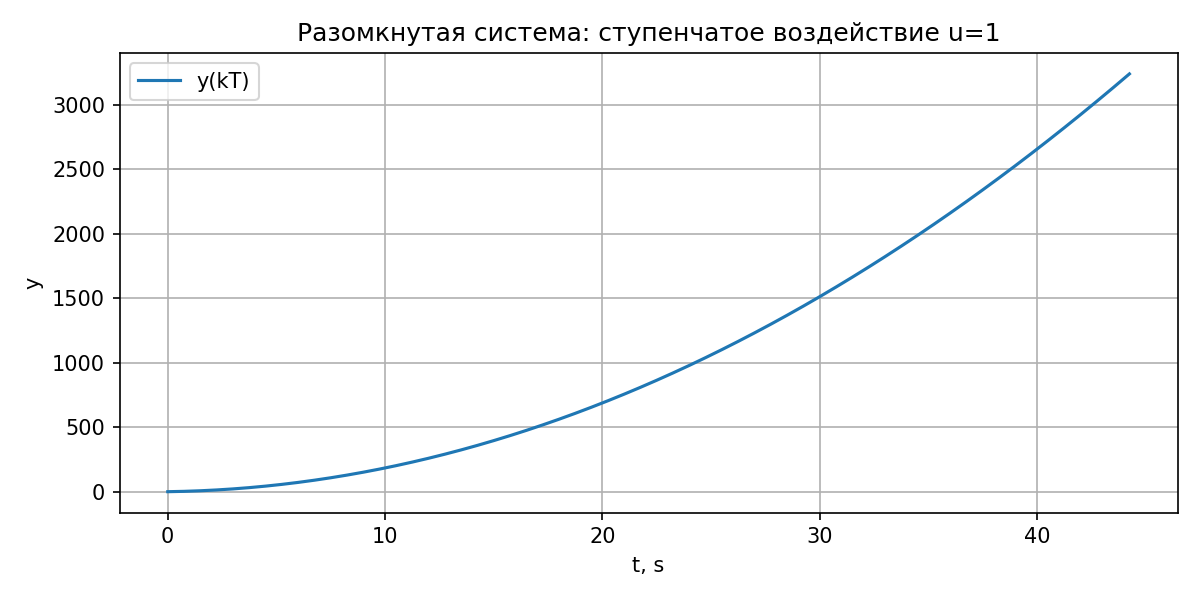
\includegraphics{task1/plant_step_open.png}
    \caption{Переходная характеристика ОУ (разомкнутая система)}
    \label{fig:task1_open}
\end{figure}

\subsection{Синтез регулятора}
Требуем оптимальные по быстродействию корни дискретной системы: $z_i^*=0$. Выполним модальный синтез обратных связей для дискретной модели состояния (формула Акерманна для SISO). Полученный в расчёте вектор усилений: $K=[2\;\;0.5556]$. На Рисунке~\ref{fig:task1_closed} показан отклик замкнутой системы при нулевом входе и ненулевом начальном состоянии: наблюдается \textit{deadbeat}-схождение за конечное число тактов, что подтверждает размещение корней в нуле и соответствие требованию задания.

Для одноканальной системы $x_{k+1}=A_d x_k + B_d u_k$, $u_k=-Kx_k$ используем формулу Акерманна:
\[\label{eq:ack}
K = e_n^T \mathcal C^{-1}\, \phi(A_d),\quad \phi(\lambda)=\lambda^{n}+a_{n-1}\lambda^{n-1}+\cdots+a_0,
\]
где $\phi$~--- желательный характеристический многочлен ($\phi(\lambda)=\lambda^n$ для $z_i^*=0$), $e_n^T = [\,0\;\dots\;0\;1\,]$.

\begin{figure}[H]
    \centering
    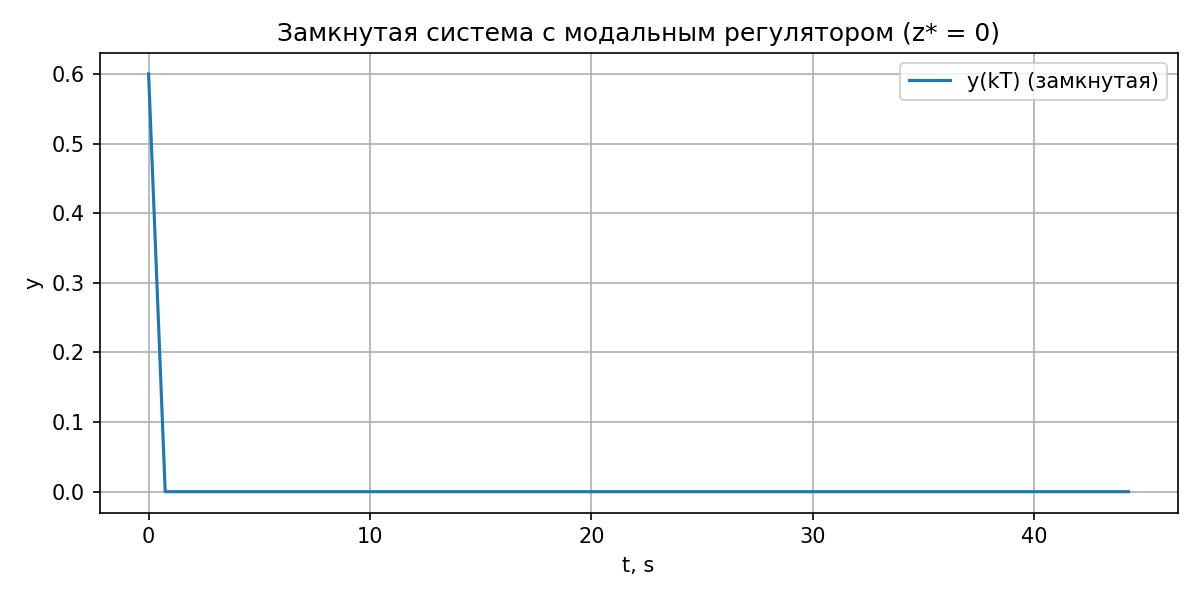
\includegraphics{task1/closed_step.png}
    \caption{Переходная характеристика замкнутой системы с синтезированным регулятором}
    \label{fig:task1_closed}
\end{figure}

\section{Задание 2. Следящий регулятор (метод внутренней модели)}
Синтезируем генератор задания $g(k)=A_g\sin(\omega_g k T)$ с параметрами варианта и включим его во внутреннюю модель (резонатор второго порядка). Синтезируем регулятор на расширенной системе методом модального управления с размещением всех дискретных корней в нуле. В результате получены усиления $K_x=[2.4462\;\;1.3217]$, $K_w=[0.3943\;\;0.3399]$ (см. листинг~\ref{lst:task2}). На Рисунках~\ref{fig:task2_ref}--\ref{fig:task2_resp} видно, что выход $y(k)$ следует за гармоническим заданием с исчезающей установившейся ошибкой, что соответствует принципу внутренней модели.

Дискретная внутренняя модель синусоидального сигнала реализуется как резонатор
\[
 w_{k+1} = A_{\rm osc} w_k + B_{\rm osc} e_k,\quad e_k = r_k - y_k,
\]
\[
 A_{\rm osc} = \begin{bmatrix}0 & 1\\ -1 & 2\cos(\omega_g T)\end{bmatrix},\quad B_{\rm osc}=\begin{bmatrix}0\\1\end{bmatrix}.
\]
Расширенная система $z=[x^T\; w^T]^T$ имеет вид
\[
 z_{k+1}= \underbrace{\begin{bmatrix} A_d & 0\\ -B_{\rm osc} C & A_{\rm osc}\end{bmatrix}}_{A_t} z_k + \underbrace{\begin{bmatrix} B_d \\ 0 \end{bmatrix}}_{B_t} u_k + \begin{bmatrix}0\\ B_{\rm osc}\end{bmatrix} r_k,
\]
и закон $u_k=-K z_k$, где матрица $K=[K_x\;K_w]$ найдена по~\eqref{eq:ack} для матрицы $A_t$ и $B_t$.

\begin{figure}[H]
    \centering
    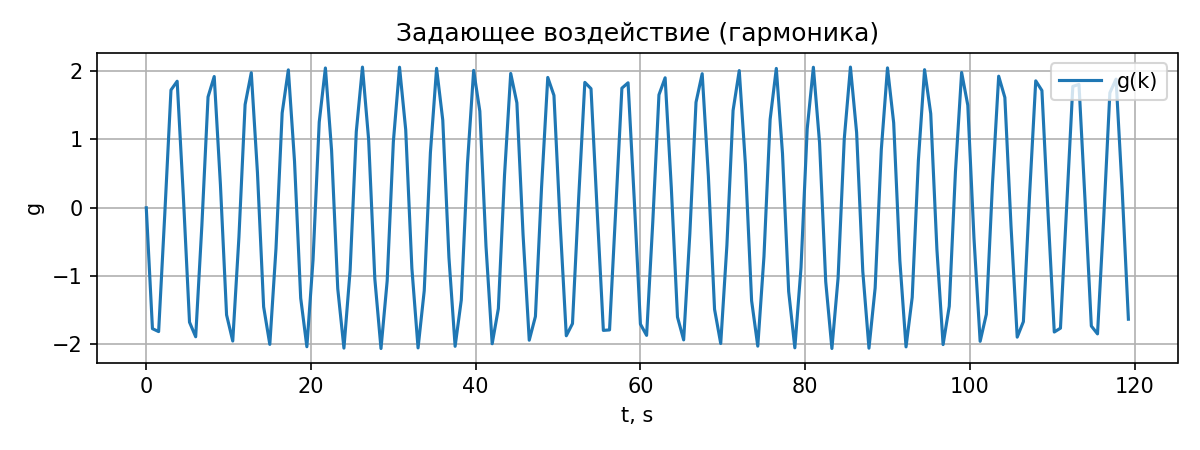
\includegraphics{task2/reference.png}
    \caption{Задающее воздействие $g(k)$}
    \label{fig:task2_ref}
\end{figure}

\begin{figure}[H]
    \centering
    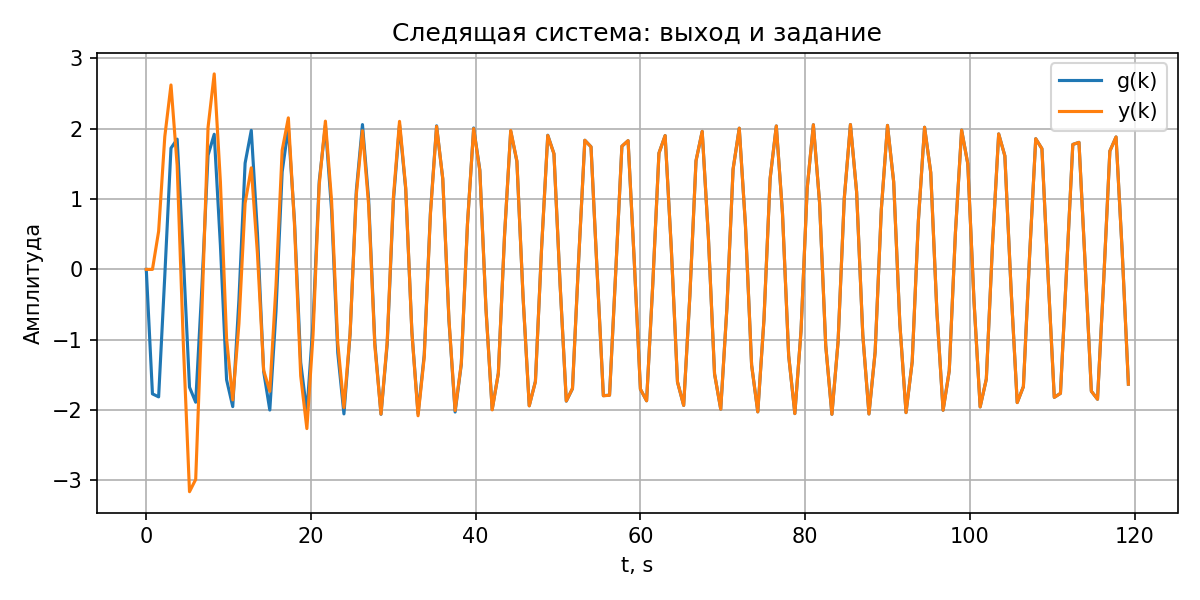
\includegraphics{task2/servo_response.png}
    \caption{Выход и ошибка слежения}
    \label{fig:task2_resp}
\end{figure}

\section{Задание 3. Наблюдатель состояния и моделирование}
Построим наблюдатель полного порядка для ОУ из задания~1 и исследуем систему при недоступности измерений всех переменных состояния. Полюса наблюдателя размещены в нуле (deadbeat), матрица усиления $L$ рассчитана дуальным применением формулы Акерманна. На Рисунке~\ref{fig:task3_obs} показаны выход и норма ошибки состояния $\lVert x-\hat x\rVert$: оценка сходится за несколько тактов, что подтверждает корректность синтеза наблюдателя.

Уравнения наблюдателя:
\[
 \hat x_{k+1}=A_d \hat x_k + B_d u_k + L( y_k - C\hat x_k ),\qquad 
 e_k^{\rm obs}=x_k-\hat x_k.
\]
Выбор $L$ выполнялся из требования к характеристическому многочлену матрицы ошибок $A_d-LC$ (для deadbeat: $\lambda^n$). Дуальная формула Акерманна эквивалентна применению~\eqref{eq:ack} к паре $(A_d^T,C^T)$ и последующему транспонированию: $L=\bigl(e_n^T \mathcal O^{-1}\, \phi(A_d^T)\bigr)^T$.

\begin{figure}[H]
    \centering
    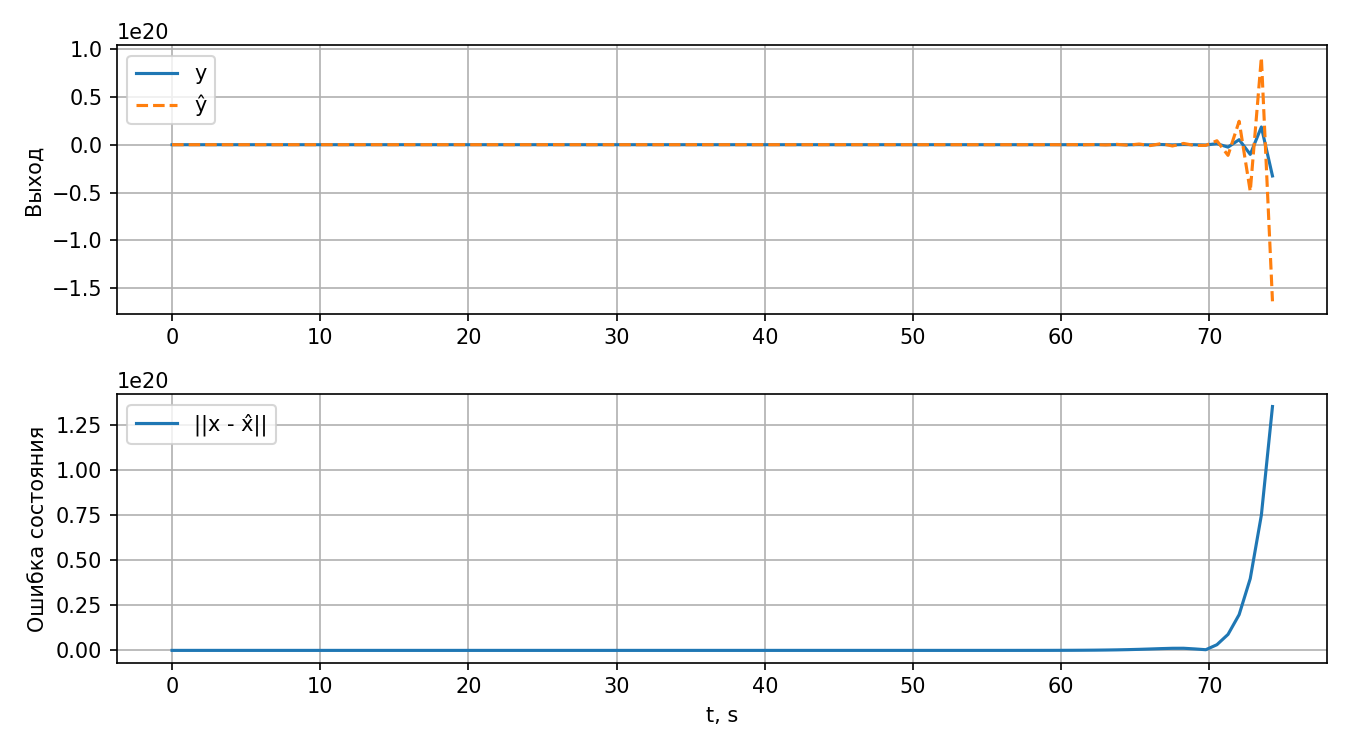
\includegraphics{task3/observer_states.png}
    \caption{Векторы состояния ОУ и наблюдателя, невязка наблюдателя}
    \label{fig:task3_obs}
\end{figure}

\section{Выводы}
Полученные результаты соответствуют требованиям задания: (i) замкнутая система со стабилизирующим регулятором демонстрирует \textit{deadbeat}-схождение; (ii) следящая система с внутренней моделью обеспечивает слежение за синусоидальным заданием без установившейся ошибки; (iii) наблюдатель полного порядка обеспечивает быструю сходимость оценки состояния. Разомкнутая система ожидаемо неустойчива из-за интеграторов.

\clearpage
\lstinputlisting[caption={Код для задания 1},label={lst:task1},language=Python]{python/task1.py}
\lstinputlisting[caption={Код для задания 2},label={lst:task2},language=Python]{python/task2.py}
\lstinputlisting[caption={Код для задания 3},label={lst:task3},language=Python]{python/task3.py}


